\documentclass{article}\usepackage[]{graphicx}\usepackage[]{color}
% maxwidth is the original width if it is less than linewidth
% otherwise use linewidth (to make sure the graphics do not exceed the margin)
\makeatletter
\def\maxwidth{ %
  \ifdim\Gin@nat@width>\linewidth
    \linewidth
  \else
    \Gin@nat@width
  \fi
}
\makeatother

\definecolor{fgcolor}{rgb}{0.345, 0.345, 0.345}
\newcommand{\hlnum}[1]{\textcolor[rgb]{0.686,0.059,0.569}{#1}}%
\newcommand{\hlstr}[1]{\textcolor[rgb]{0.192,0.494,0.8}{#1}}%
\newcommand{\hlcom}[1]{\textcolor[rgb]{0.678,0.584,0.686}{\textit{#1}}}%
\newcommand{\hlopt}[1]{\textcolor[rgb]{0,0,0}{#1}}%
\newcommand{\hlstd}[1]{\textcolor[rgb]{0.345,0.345,0.345}{#1}}%
\newcommand{\hlkwa}[1]{\textcolor[rgb]{0.161,0.373,0.58}{\textbf{#1}}}%
\newcommand{\hlkwb}[1]{\textcolor[rgb]{0.69,0.353,0.396}{#1}}%
\newcommand{\hlkwc}[1]{\textcolor[rgb]{0.333,0.667,0.333}{#1}}%
\newcommand{\hlkwd}[1]{\textcolor[rgb]{0.737,0.353,0.396}{\textbf{#1}}}%
\let\hlipl\hlkwb

\usepackage{framed}
\makeatletter
\newenvironment{kframe}{%
 \def\at@end@of@kframe{}%
 \ifinner\ifhmode%
  \def\at@end@of@kframe{\end{minipage}}%
  \begin{minipage}{\columnwidth}%
 \fi\fi%
 \def\FrameCommand##1{\hskip\@totalleftmargin \hskip-\fboxsep
 \colorbox{shadecolor}{##1}\hskip-\fboxsep
     % There is no \\@totalrightmargin, so:
     \hskip-\linewidth \hskip-\@totalleftmargin \hskip\columnwidth}%
 \MakeFramed {\advance\hsize-\width
   \@totalleftmargin\z@ \linewidth\hsize
   \@setminipage}}%
 {\par\unskip\endMakeFramed%
 \at@end@of@kframe}
\makeatother

\definecolor{shadecolor}{rgb}{.97, .97, .97}
\definecolor{messagecolor}{rgb}{0, 0, 0}
\definecolor{warningcolor}{rgb}{1, 0, 1}
\definecolor{errorcolor}{rgb}{1, 0, 0}
\newenvironment{knitrout}{}{} % an empty environment to be redefined in TeX

\usepackage{alltt}
\title{Statistical Programming with R\\Assignment 2}

\author{\small Tove Henning\\ \small Carl Munkby\\ \small Johannes Zetterberg}
\date{}

\usepackage[margin = 1in]{geometry}
\IfFileExists{upquote.sty}{\usepackage{upquote}}{}
\begin{document}
\maketitle

\pagebreak

\section{Least squares variance simulation}

In linear regression, given that the Gauss-Markov theorem is satisfied, ordinary least squares is considered (OLS) to be the best linear unbiased estimator. If the assumption of homoscedasticity is violated, then OLS won’t be the estimator with the smallest variance (the most efficient). Instead, to handle heteroscedasticity, one could make use of a weighted least squares estimator (WLS), which can be more efficient than OLS. The weights in WLS can be constructed easily if the variance is known. If the variance is unknown it is still possible to perform WLS but a certain parametric structure needs to be assumed, this method is called feasible weighted least squares (FWLS).


In the following section a comparison between the three different methods will be carried out. The goal is to see how they differ in terms of efficiency by performing estimation based on simulated data.



\subsubsection*{Ordinary least squares}

To estimate the beta for the ordinary least squares estimator we used the two vector dataset and set column one to \textbf{y} and column two to \textbf{X}, where \textbf{y} is the dependent variable and \textbf{X} the explanatory variable. Adding an extra intercept column of n rows to \textbf{X}. Lastly a calculation of the ordinary least squares estimator has been done by using the formula:
$\hat{\beta}_{OLS}=(\textbf{X}’\textbf{X})^{-1}\textbf{X}’\textbf{y}$.



\subsubsection*{Weighted least squares}

To estimate the beta for the weighted least squares estimator we used the two vector dataset and set column one to \textbf{y} and column two to \textbf{X}, where \textbf{y} is the dependent variable and \textbf{X} the explanatory variable. Then an extra intercept column of n rows has been added to \textbf{X}. To be able to get the error covariance matrix $\omega$ we added a zero matrix of size n x n. By running a for loop where the exponent of \textbf{X} times $\lambda$ is added on the diagonal in the zero matrix calculates our $\omega$. The value of the weighted least square estimator is then computed by: 
$\hat{\beta}_{WLS}=(\textbf{X}’\Omega({\lambda})^{-1}\textbf{X})^{-1}\textbf{X}’\Omega({\lambda})^{-1}\textbf{y}$.




\subsubsection*{Feasible weighted least squares}

To estimate beta for the feasible weighted least squares estimator we needed to assume some structure for the error variance depending on whether the variance form is true ($\sigma^2_{\epsilon_i} = e^{x_i\lambda}$) or false ($\sigma^2_{\epsilon_i} = 1 + x_i\lambda$). The data is divided into \textbf{y} and \textbf{X}, \textbf{y} being the dependent variable, \textbf{X} being the explanatory variable. A linear regression model of \textbf{y} and \textbf{X} is estimated and the residuals from this model are used to estimate another linear regression model. In this model, the dependent variable is the natural logarithm of the squared residuals and the independent variable is \textbf{X}. The coefficient of this linear model is the estimated value of $\lambda$, that is, $\hat{\lambda}$. This value of $\hat{\lambda}$ is then used to get an estimate of the error covariance matrix $\Omega(\hat{\lambda})$, where the diagonal is filled with the value of the estimated error variance for each value of x, $\hat{\sigma}^2_{\epsilon_i}$, which differs depending on whether the variance form is assumed to be true of false. 
The value of the feasible weighted least squares estimator is then computed by: $\hat{\beta}_{FWLS}=(\textbf{X}’\Omega(\hat{\lambda})^{-1}\textbf{X})^{-1}\textbf{X}’\Omega(\hat{\lambda})^{-1}\textbf{y}$.




\subsubsection*{Data}

To generate data the DataFun function was generated. It generates random data with an error term dependent on the covariance structure $   \lambda $ and the number of observations chosen. The function starts by generating the standard deviation of epsilon since the error term is dependent on x, which comes from a uniform distribution. When all the parameters are calculated the function calculates y and then all the different values of y and x are saved in a matrix and that matrix is set to be the return value.



\subsubsection*{Simulation}

The function SimFun uses all the pre-existing functions to generate data and fit models depending on the number of simulations one wants to perform. The function then returns all the fitted betas from all of the models. Except the number of simulations one can also freely choose the number of observations for the data as well, the seed number and the value of $\lambda$ .

\begin{knitrout}
\definecolor{shadecolor}{rgb}{0.969, 0.969, 0.969}\color{fgcolor}
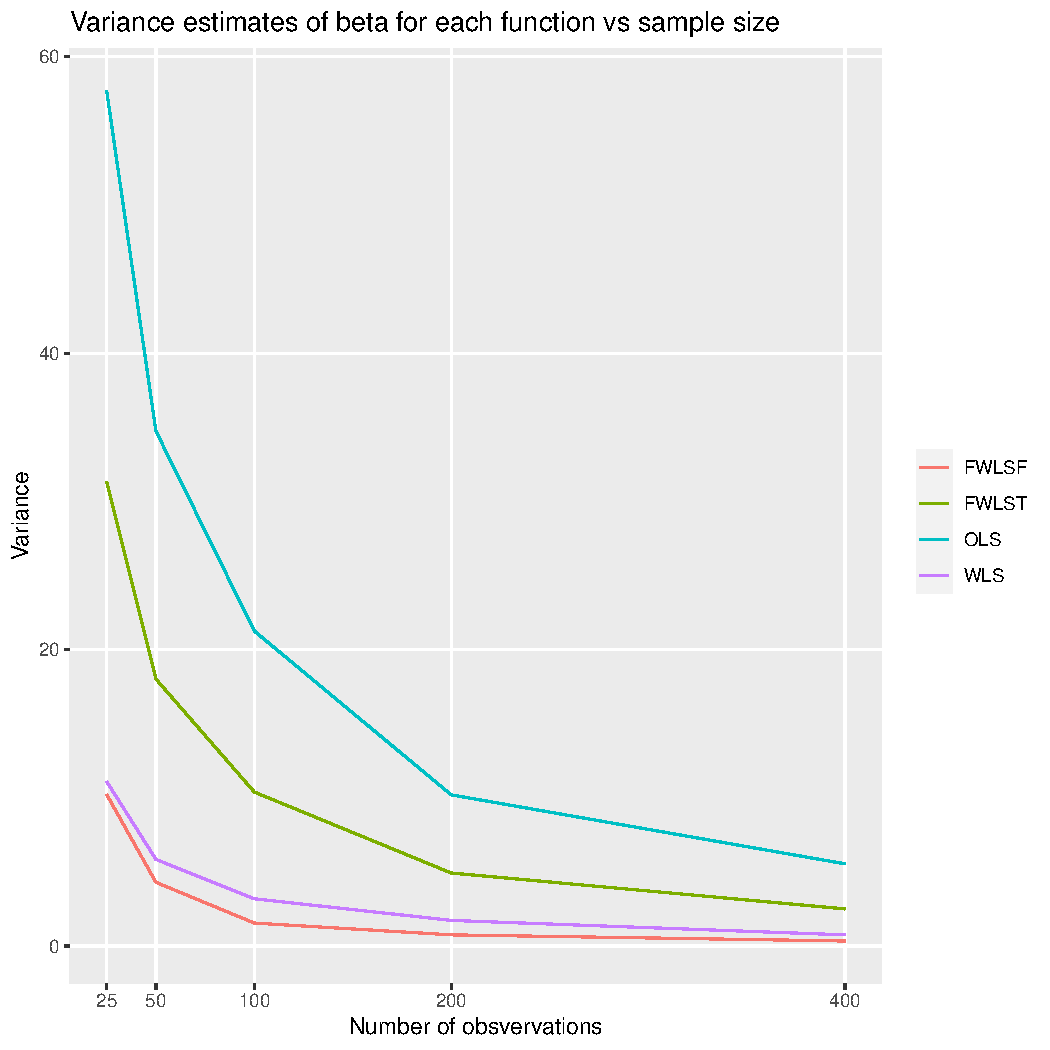
\includegraphics[width=\maxwidth]{figure/unnamed-chunk-6-1} 

\end{knitrout}

\subsection*{Figure 1: Difference in variance for the different estimators}

In figure 1 the variance estimates for each beta coefficient for different sample sizes is presented. We can see that the variance decreases for all beta estimates the larger the sample size is. The feasible least squares estimates the lowest variance both when the variance form is true and false, i.e. is the most efficient estimator. We can say that the FWLS is BLUE. The plot clearly shows that OLS is inefficient, it looks to lack heteroscedasticity since the variance differs much depending on sample size. WLS is better than OLS but still has some bias.

\pagebreak

\section{EM algorithm for mixture of normals}

Real world data can tend to come in shapes of clusters meaning that the normal distribution won’t be suitable for describing the generation of observations. However the normal distribution could still be utilized but as a linear combination with one distribution for every cluster (K). The expectation-maximation (EM) algorithm is a useful method for finding the maximum likelihood estimates for a mixture of normal models.

In the following section an example of an implementation of the EM algorithm on the dataset galaxies will be carried out. As for all clustering problems the question of the suiting number of clusters seldom has a clear cut answer and often requires further investigation. 

\begin{knitrout}
\definecolor{shadecolor}{rgb}{0.969, 0.969, 0.969}\color{fgcolor}
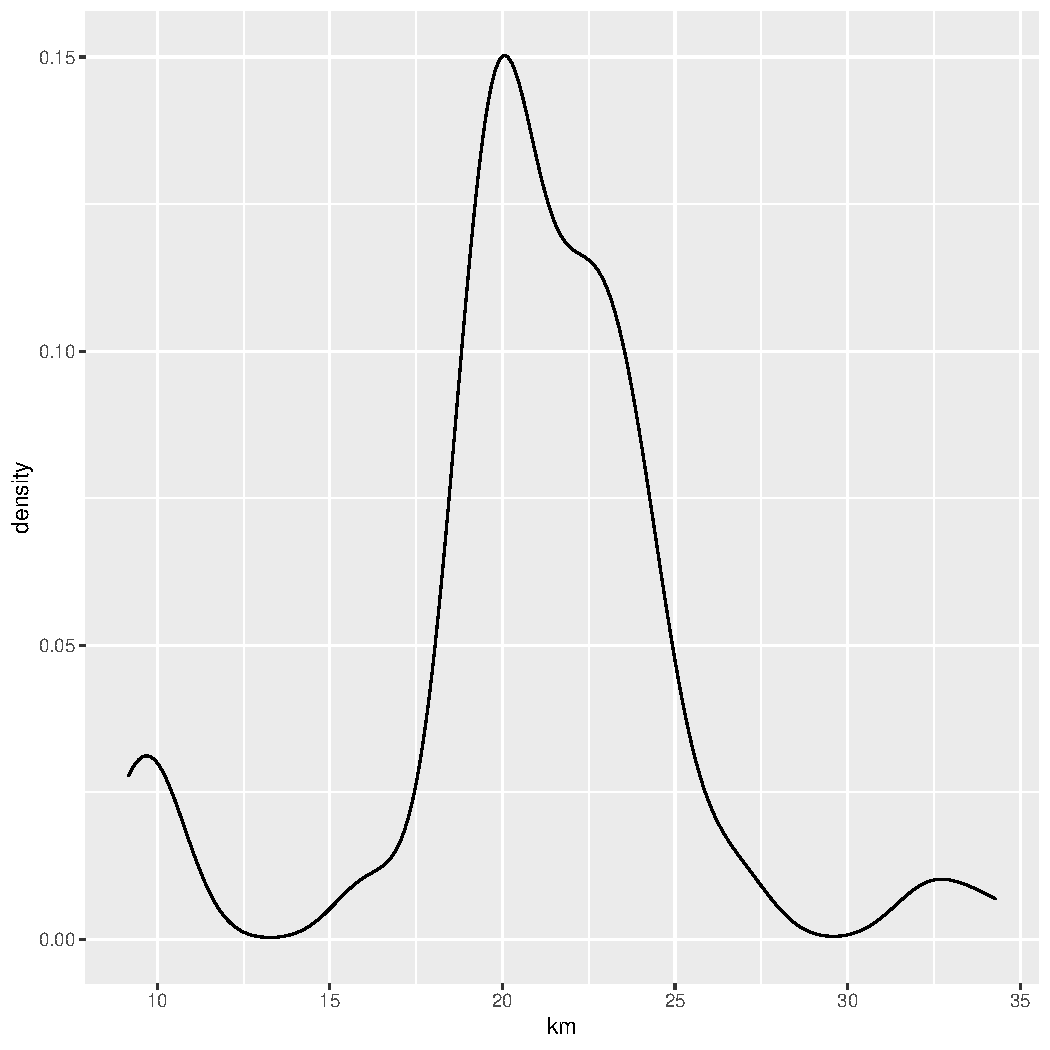
\includegraphics[width=\maxwidth]{figure/unnamed-chunk-7-1} 

\end{knitrout}

\subsection*{Figure 2: Distribution of the raw data}

In figure 2 we can see a density plot of the data set galaxies. By examining the plot we think that three groups would be suitable to describe the data, first group that covers the area around 10 km, second in the larger area in the middle, and third that has its mean between 30 and 35 km.

\subsection*{Implementing the steps with functions}

To be able to practically implement the EM-algorithm, several functions are created. Below follows a description of all the functions used.



\subsubsection*{gammaUpdate}
The gammaUpdate function computes the E step in the EM function, that is computes the updates of $ \gamma(z_{nk})  $. The input of the function is a data set, in this case the galaxies data, and the values of sigma, mu and pi. The function then returns a $n \cdot  K$ matrix of $\gamma{z_{nk}}  $  values, where n is the number of observations in the galaxies data and K is the number of clusters. In this return, every row sums to 1.



\subsubsection*{muUpdate}

The muUpdate function takes a data variable and a gamma variable as input and then calculates and returns a new $\mu$ for all of the clusters.



\subsubsection*{sigmaUpdate}
The sigmaUpdate function takes a data variable and the values of gamma and mu as input and calculates and returns a new $\sigma_k$ for each cluster.  



\subsubsection*{piUpdate}

The piUpdate function takes a gamma variable as input and then calculates and returns a new $\pi$ for all clusters.



\subsubsection*{loglik}
The loglik-function computes the log-likelihood of the data for given parameters. The function takes the galaxies data and value of pi, mu and sigma as input and then calculates the log-likelihood by looping through the clusters and the rows in the input data. The function then returns the log-likelihood.



\subsubsection*{initialValues}

The initialValues function randomly computes the initial values for $\mu$, $\sigma$ and $\pi$ and computes the initial log-likelihood. It repeats this process 100 times and only saves the values if the new log-likelihood is higher than the last one. The function returns $\mu$, $\sigma$, $\pi$ and the log-likelihood.



\subsubsection*{EM}

The EM function combines all the pre-existing functions and performs the full EM-algorithm. First it initializes some starting values for $\mu$, $\sigma$ and $\pi$ and computes the initial log-likelihood (step 1). It then computes $\gamma$ (step 2), re-estimates the parameters (step 3) and evaluates the new log-likelihood (step 4). By the use of a while loop step 2 to step 4 is repeated until the absolute change in log-likelihood is less than 0.001. The function takes in a vector of data points and a variable with a value corresponding to the desired number of clusters. The function returns a list containing the values of log-likelihood, the mean, the standard deviation and the partitions of the clusters.

\begin{knitrout}
\definecolor{shadecolor}{rgb}{0.969, 0.969, 0.969}\color{fgcolor}
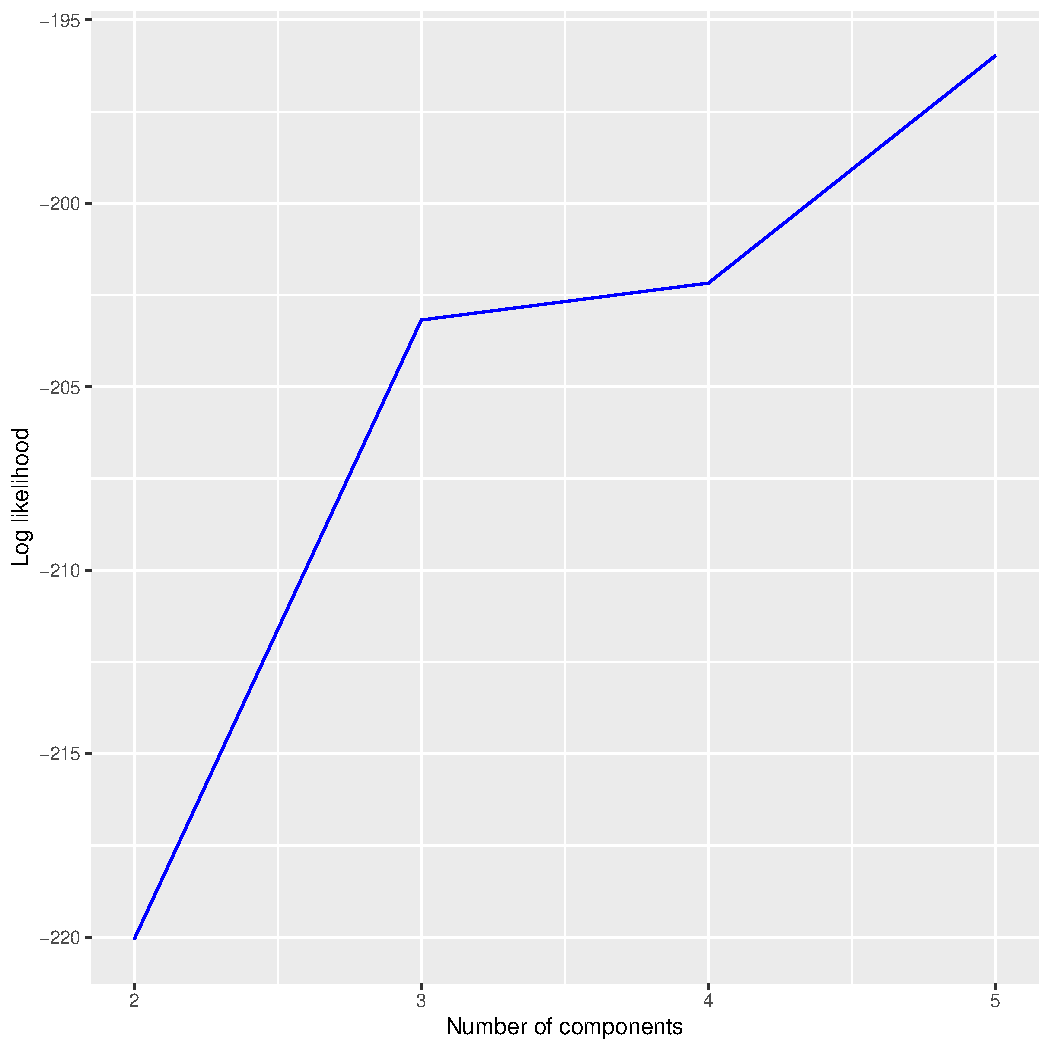
\includegraphics[width=\maxwidth]{figure/unnamed-chunk-15-1} 

\end{knitrout}

\subsection*{Figure 3: Log likelihood for each number of components}

In figure 3 we can see the number of components and their respective log likelihoods. The results show that the log likelihood increases as the number of components K increases. It is very reasonable that the likelihood increases as the number of partitions increases but it won’t be very useful to solely focus on the value of the log likelihood. Too many clusters won’t be practical instead it would be more appropriate to focus on the marginal increase in log-likelihood as the number of components increases. The plot shows that the marginal increase in log-likelihood stagnates after 3 components motivating the choice of 3 clusters. However since initial values in the EM-algorithm are generated randomly the local log-likelihood optimums may differ meaning that if we were to re-apply the EM-algorithm we would possibly observe different gradients in the plot.

\begin{knitrout}
\definecolor{shadecolor}{rgb}{0.969, 0.969, 0.969}\color{fgcolor}
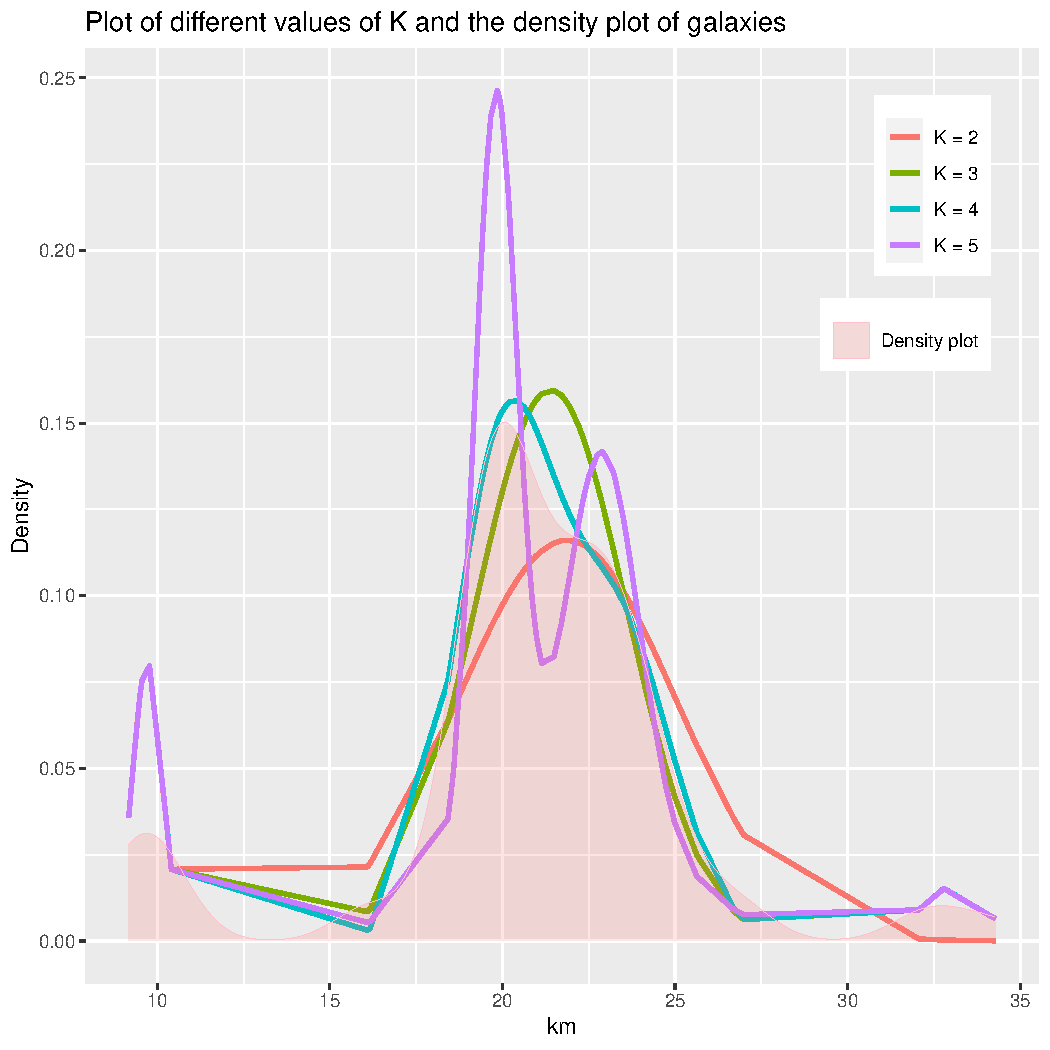
\includegraphics[width=\maxwidth]{figure/unnamed-chunk-16-1} 

\end{knitrout}

\subsection{Figure 4: Plot of different values of K and the density plot of galaxies}

In figure 4 a comparison for different values of K, components, when running the EM algorithm is presented. When comparing the density plot with all the distributions the model with 4 partitions seems to fit the data best. However, when looking back at figure 3, we see that the increase in log-likelihood is very small when going from 3 to 4 components. Keeping in mind that the number of observations are quite low in this dataset, a partition of 3 is argueably more suitable since a partition of 4 or higher may run the risk of resulting in overfitting. 

\end{document}
